% !TEX root = ../thesis-example.tex
%
\chapter{Architecture of Chrysalis}
\label{sec:init}

Since \emph{Chrysalis} was handed to us as an already running prototype including a predefined layer structure and a way to interact with it in a browser, those designs were therefore a given. The Application is written entirely in JavaScript code, with the code deployed to the Blockchains sometimes being an exception.
The prototype version was able to run on an \emph{Ethereum}-Blockchain-Network, demonstrating it's functionality.
In this chapter, we elaborate on the general structure of \emph{Chrysalis}, omitting technical details and focusing on how the user and the components interact.

\section{Intended Usage}
\label{sec:init:usage}

From the user's point of view, three interactions with the system are generally intended, as they're described below. The configuration aside, the other two, encapsulating BPM, are shown in figure \ref{fig:init:usage:bpm}.

\begin{figure}[h]
	\centering
	\captionsetup{justification=centering,margin=2cm}
	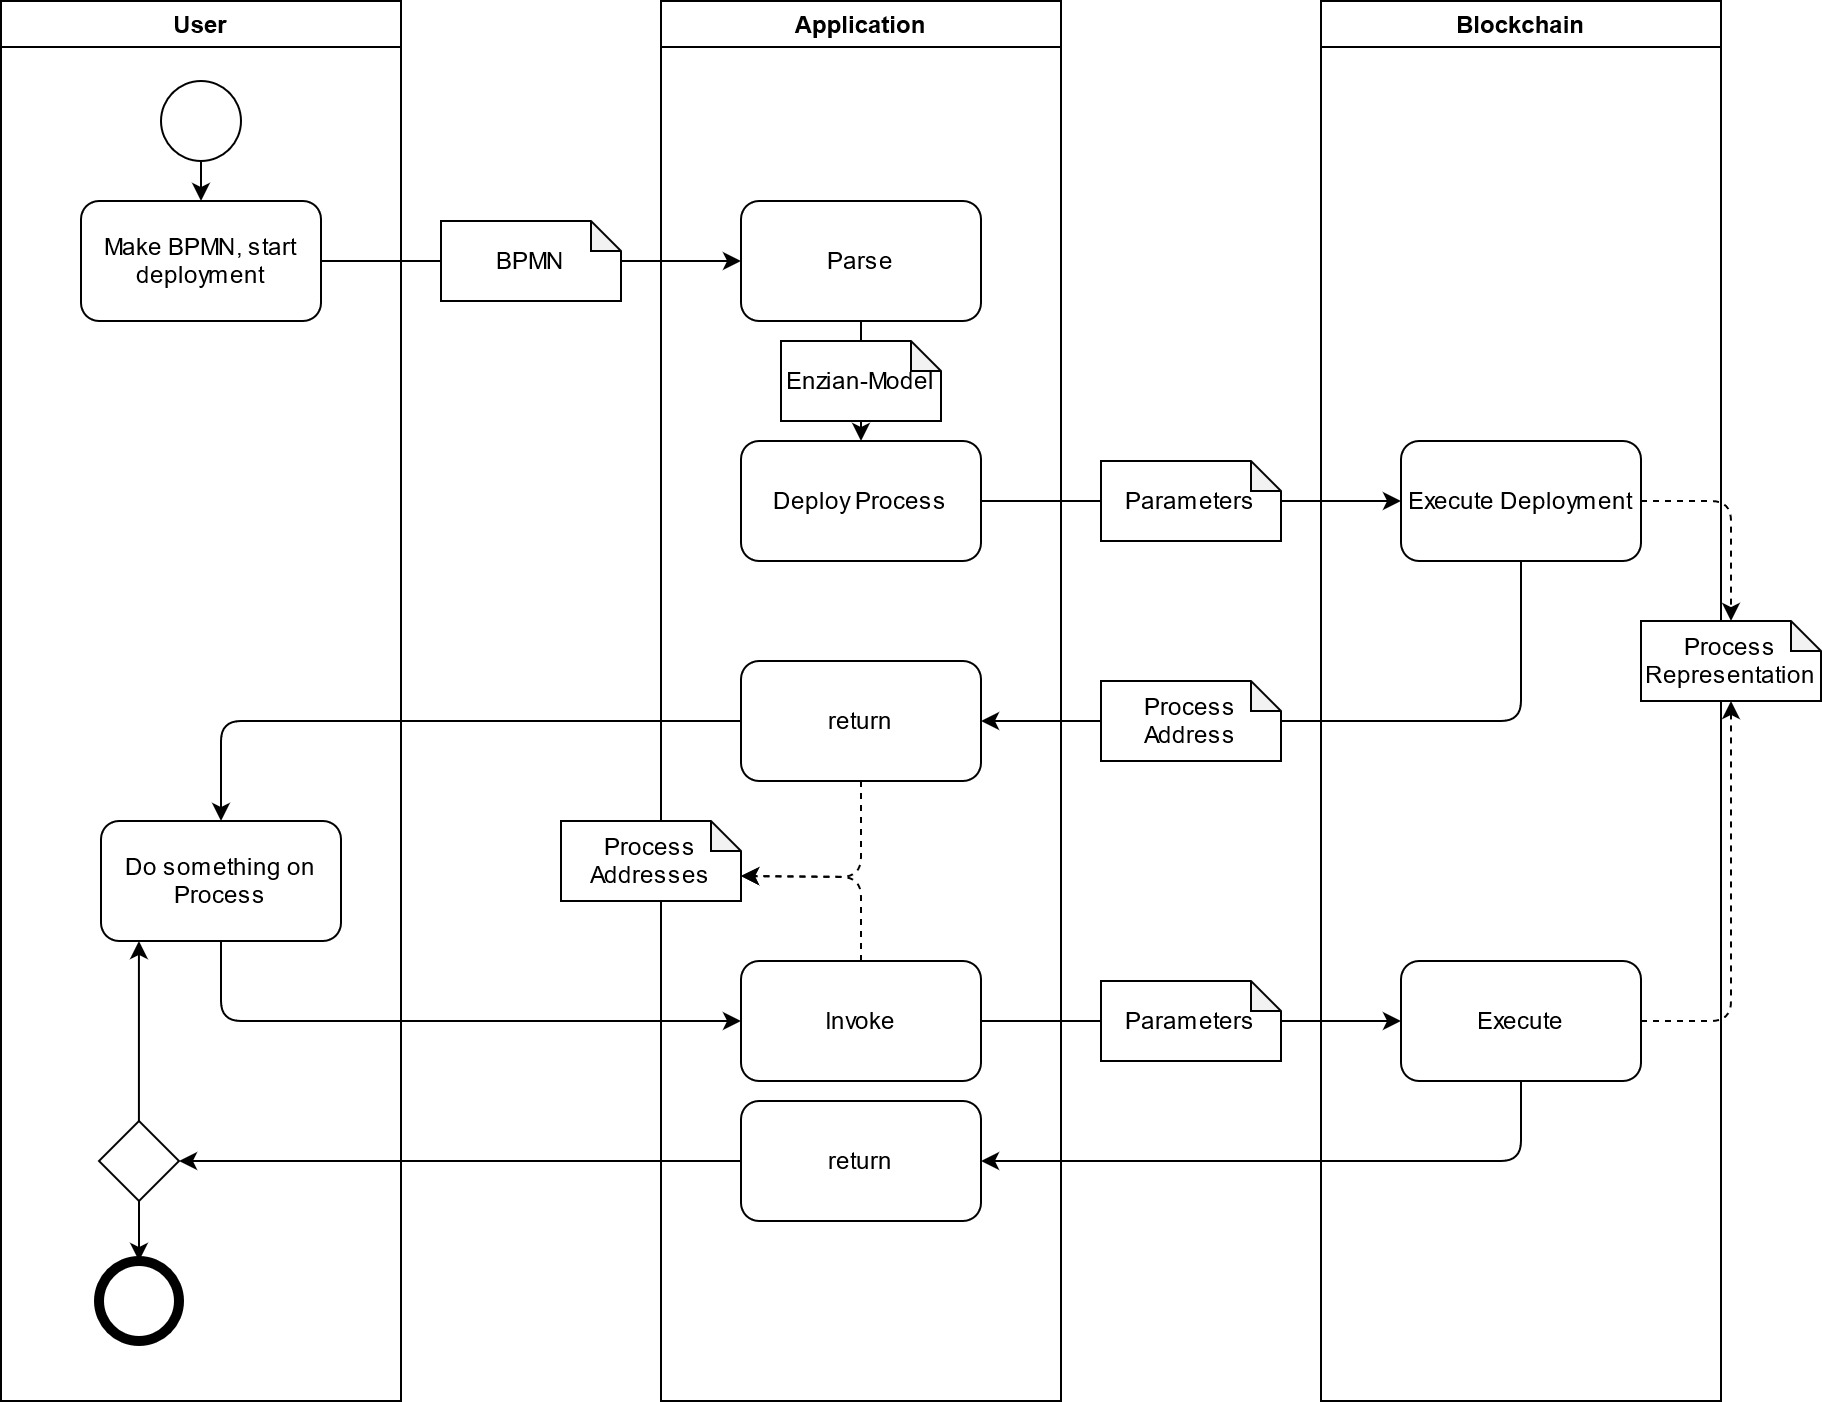
\includegraphics[height=0.7\textwidth]{gfx/bpmn2bc}
	\caption{Workflow and artifacts created during process deployment and execution.}
	\label{fig:init:usage:bpm}
\end{figure}

\textbf{Configuration} \\[0.2em]
Before BPM actions are possible, some parameters must be set. First, the endpoint URL of the local Blockchain application (the Blockchain \emph{node}) must be declared. Additionally, the authentication of the user before the node is needed, usually a private key or cryptographic token of the likes. In the case of the original \emph{Chrysalis} application, the browser plugin \emph{Metamask} could also be used to provide these credentials, with the app automatically detecting the plugin and using it's connections.

\textbf{Process Deployment} \\[0.2em]
For instantiating a process, first and foremost the user needs to provide the underlying process model. This is done by handing over a file written in BPMN format containing the model. Additionally, the user selects where to deploy said process - usually the previously configured private network - and via which interface the Blockchain application shall be contacted. Then, the user simply hits the 'Deploy' button and the application handles the rest, parsing and deploying the provided model to the provided target, returning and saving the address where the process instance is situated on the blockchain data structure.

\textbf{Process Execution} \\[0.2em]
Given a deployed process's address, the user can then switch to the execution tab, where they may select the process and specify the task they wish to execute. All other details of the execution are handled in the background. At the beginning and after every task execution, the user will also see the current event log of the selected process instance, getting feedback about the current process state. This is currently the only way of telling whether a process might be executable.

\section{Components and their Interactions}
\label{sec:init:components}


\begin{figure}[h]
	\centering
	\captionsetup{justification=centering,margin=2cm}
	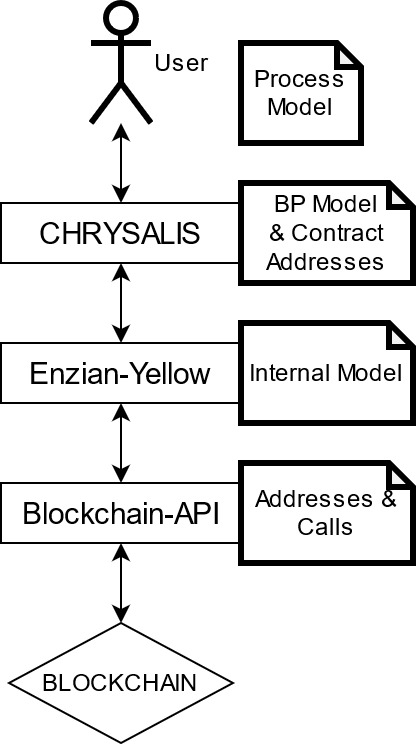
\includegraphics[height=0.5\textwidth]{gfx/init-components-layers}
	\caption{Layer structure of the original \emph{Chrysalis} System.}
	\label{fig:init:components:layers}
\end{figure}

The name-giving component, \emph{Chrysalis}, is a front-end application written in \emph{React} (for disambiguation, we will refer to this component as 'Chrysalis' and the entire system as 'project' or 'application'). While it serves as a window for the user to interact with, it also handles the storage of any relevant data, like the addresses of deployed processes and authentication credentials of the user. \emph{Chrysalis}, like any React-app, deploys a packaged version of itself and it's dependencies into the user's browser, to be executed there. As for business process interactions, it instantiates an \emph{Enzian-Yellow} object with the fitting configuration and delegates all commands to it.

\emph{Enzian-Yellow}, being an installed dependency of \emph{Chrysalis}, does the abstraction work between BPM actions and Blockchain operations. When instantiated and configured, it will instantiate and configure a Blockchain-API to connect to the corresponding network node. \emph{Enzian-Yellow} offers methods like creating and deploying processes and executing tasks, which are internally translated into the corresponding API invocations, and vice versa for the node's responses.

The \emph{Blockchain-API} is the gateway from a local program to interact with a specified Blockchain network node. When instantiated, it establishes a connection to the specified node, handles authorization and abstracts the networking away, so that the Blockchain's data and functions may be used as if they were local to the code.

The \emph{Blockchain Network Node}, depicted in figure \ref{fig:init:components:layers} as 'Blockchain', usually acts like a server that has a local copy of the Blockchain. It is fully synchronous with the network and any operation on the chain (i.e., addition of blocks) will be mirrored on every node in the network. In our case this means that every BPM action will be synchronized for every network participant that way.

\section{Modeling of Processes}
\label{sec:init:model}

To store and interact with data on the blockchain in a defined way, the Blockchains usually offer a specific gateway to guard the chain's state from abuse: \emph{Smart Contracts}, which we will also simply refer to as \emph{Contracts}. A Smart Contract is an executable program or routine written onto the Blockchain itself, so that every peer of the network may see it's definitions. This has multiple advantages in the \emph{Chrysalis} application's use case:

\begin{itemize}
    \item \emph{Transparent logic:} Since the process logic is defined in the smart contract, every peer has a transparent definition of how a process may be changed - in extension, we define that a process may never be changed outside contract definitions.
    \item \emph{Security:} Since a contract is the only way to interact with a process, every peer may check the validity of a proposed contract invocation. As peers have to agree on Blockchain interactions before they are written, the trust issue mentioned in section \ref{sec:intro} is solved.
    \item \emph{Data handling:} The smart contract either internally memorizes the location of deployed process models or translates external keys into their location. Either way, the contract abstracts memory addresses inside the Blockchain away for the user and the developer.
\end{itemize}